\section{Basisplatine}
\label{sec:basisplatine}

\todo[inline]{Bild einfügen}

\subsection{Allgemeines}
\label{sec:basisplatine-allgemeines}
Die \gls{Basisplatine} dient dazu dem \gls{Core-Modul} eine umfangreiche, moderne und jederzeit erneuerbare Peripherie bereit zu stellen, um verschiedene Anwendungskonzepte schnell und einfach evaluieren zu können. Darüber hinaus soll mit Hilfe der \gls{Basisplatine} eine Versorgung und Programmierung des \gls{Core-Modul}s möglich sein. Durch Verwendung des Arduino-Shield-Konnektors können alle am Markt verfügbaren Arduino-Shields verwendet werden, daher kann man jederzeit Hardwarekomponenten tauschen oder selbst entwickeln.

\subsection{Schnittstellen}
\label{sec:basisplatine-schnittstellen}

Die \gls{Basisplatine} verfügt über die in \fref{tab:basisplatine-schnittstellen} angegebenen Schnittstellen, welche wie in \fref{fig:basisplatine-plan} zu sehen platziert sind.

\tab{basisplatine-schnittstellen}{Schnittstellen der Basisplatine}{Schnittstellen der \gls{Basisplatine}}{|c|p{10cm}|}{
    \hline
    \textbf{Schnittstelle} & \textbf{Funktion}\\
    \hline
    USART 1 & Ansteuerung von HC-06, HC-12, \gls{USB-to-UART}-Adapter\\
    \hline
    USART 2 & Ansteuerung von ESP8266, XBee-Pro, MAX232\\
    \hline
    USART 3 & Ansteuerung von Nextion-Display\\
    \hline
    SPI 1 & \\
    \hline
    \IIC{} 1 & \\
    \hline
    SWD & Programmierung auf Basis von \gls{SWD}\\
    \hline
    ST-Link V2 & Programmierung auf Basis von \gls{SWD}\\
    \hline
    JTAG & Programmierung auf Basis von \gls{JTAG}\\
    \hline
    DE-9 Buche & Ansteuerung von Nextion-Display\\
    \hline
    Arduino-Shield-Connector & Verwendung von diversen Arduino-Shields\\
    \hline
    Audio-Shield-Connector & Verwendung des HTL-internen Audio-Shields\\
    \hline
    Singe-Wire & Ansteuerung von Piezo, Temperatursensor, LFU, IR-Sensor, BMA020, EEPROM\\
    \hline
    USB-A & Spannungsversorgung, Datentransport\\
    \hline
    USB-B & Spannungsversorgung, Datentransport\\
    \hline
}

\fig{basisplatine-plan}{Übersichtsplan der Basisplatine}{Übersichtsplan der \gls{Basisplatine}}{0.75\textwidth}{Schuh/Pictures/Basisplatine}

\subsection{Portbelegungsplan}
\label{sec:basisplatine-portbelegung}
\tabpdf{basisplatine-portbelegung}{Portbelegungsplan der Basisplatine}{Portbelegungsplan der \gls{Basisplatine}}{0.5\textwidth}{Schuh/Pictures/Basis-Portbelegung}

\subsection{Gesamtschaltung}
\label{sec:basisplatine-schaltung}
\begin{figure}[htb]
    \centering
    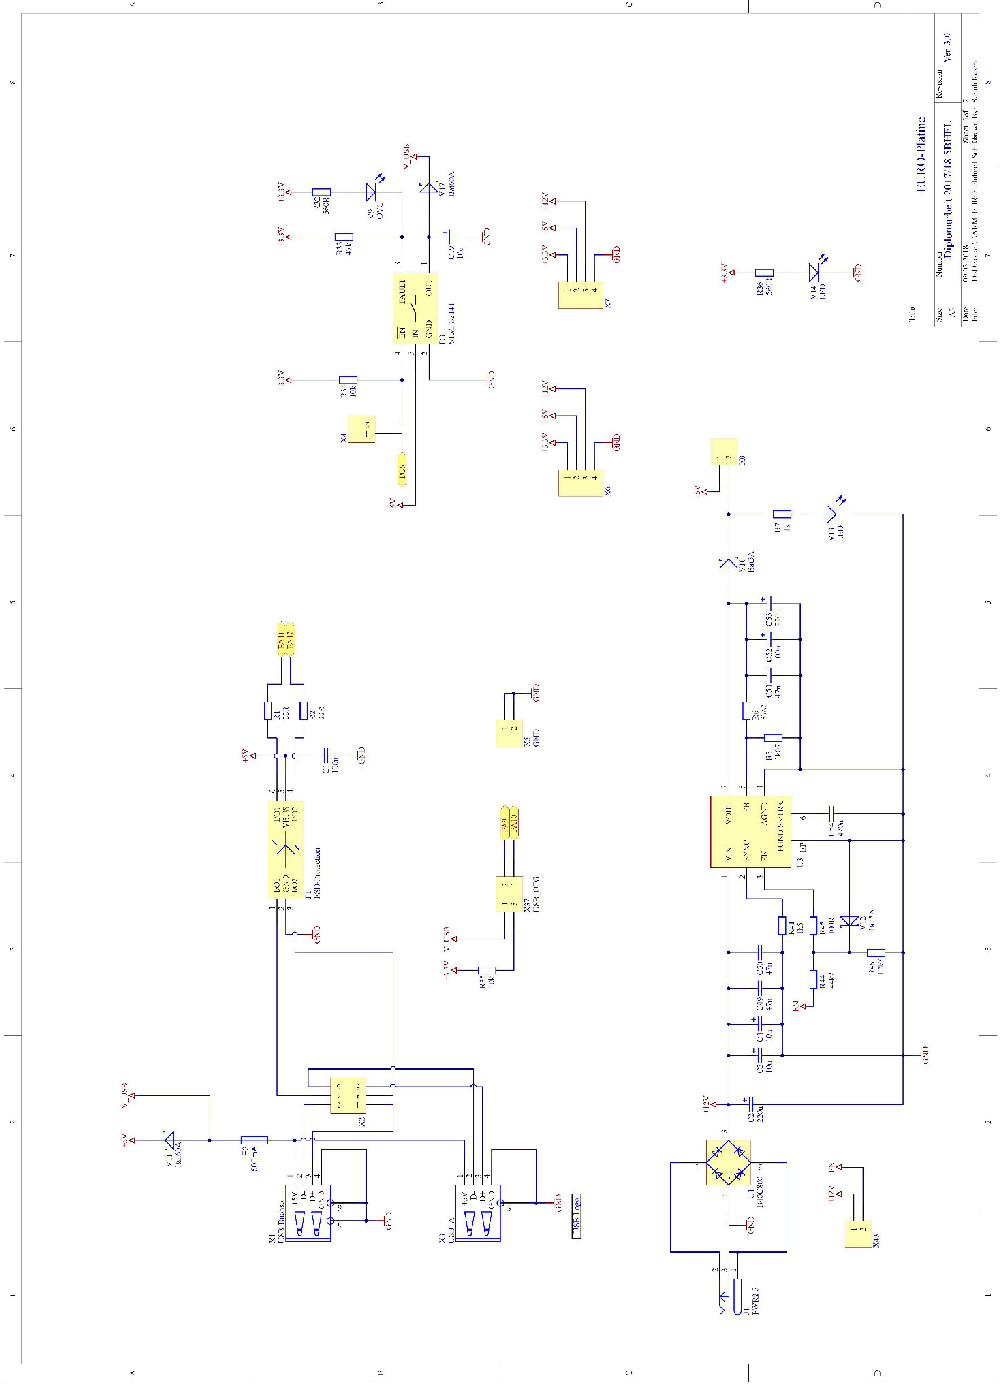
\includegraphics[width=0.8\textwidth]{Schuh/Pictures/Basis-Schaltung1}
    \caption[Gesamtschaltung der Basisplatine]{Gesamtschaltung der \gls{Basisplatine}}
    \label{fig:basisplatine-schaltung}
\end{figure}
\begin{figure}[htb]\ContinuedFloat
    \centering
    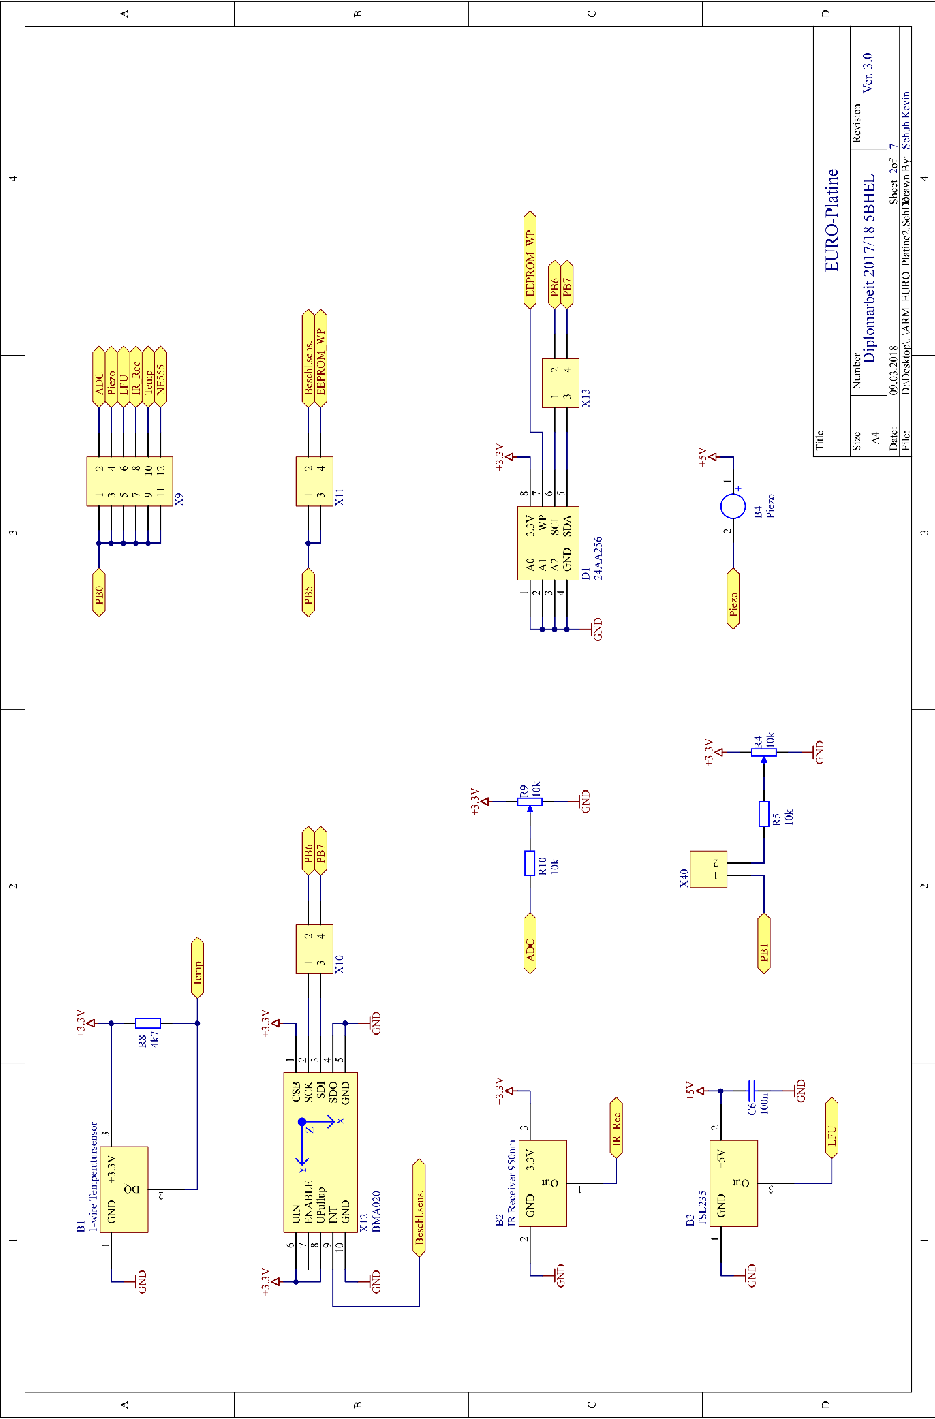
\includegraphics[width=0.8\textwidth]{Schuh/Pictures/Basis-Schaltung2}
    \caption[Gesamtschaltung der Basisplatine]{Gesamtschaltung der \gls{Basisplatine}}
\end{figure}
\begin{figure}[htb]\ContinuedFloat
    \centering
    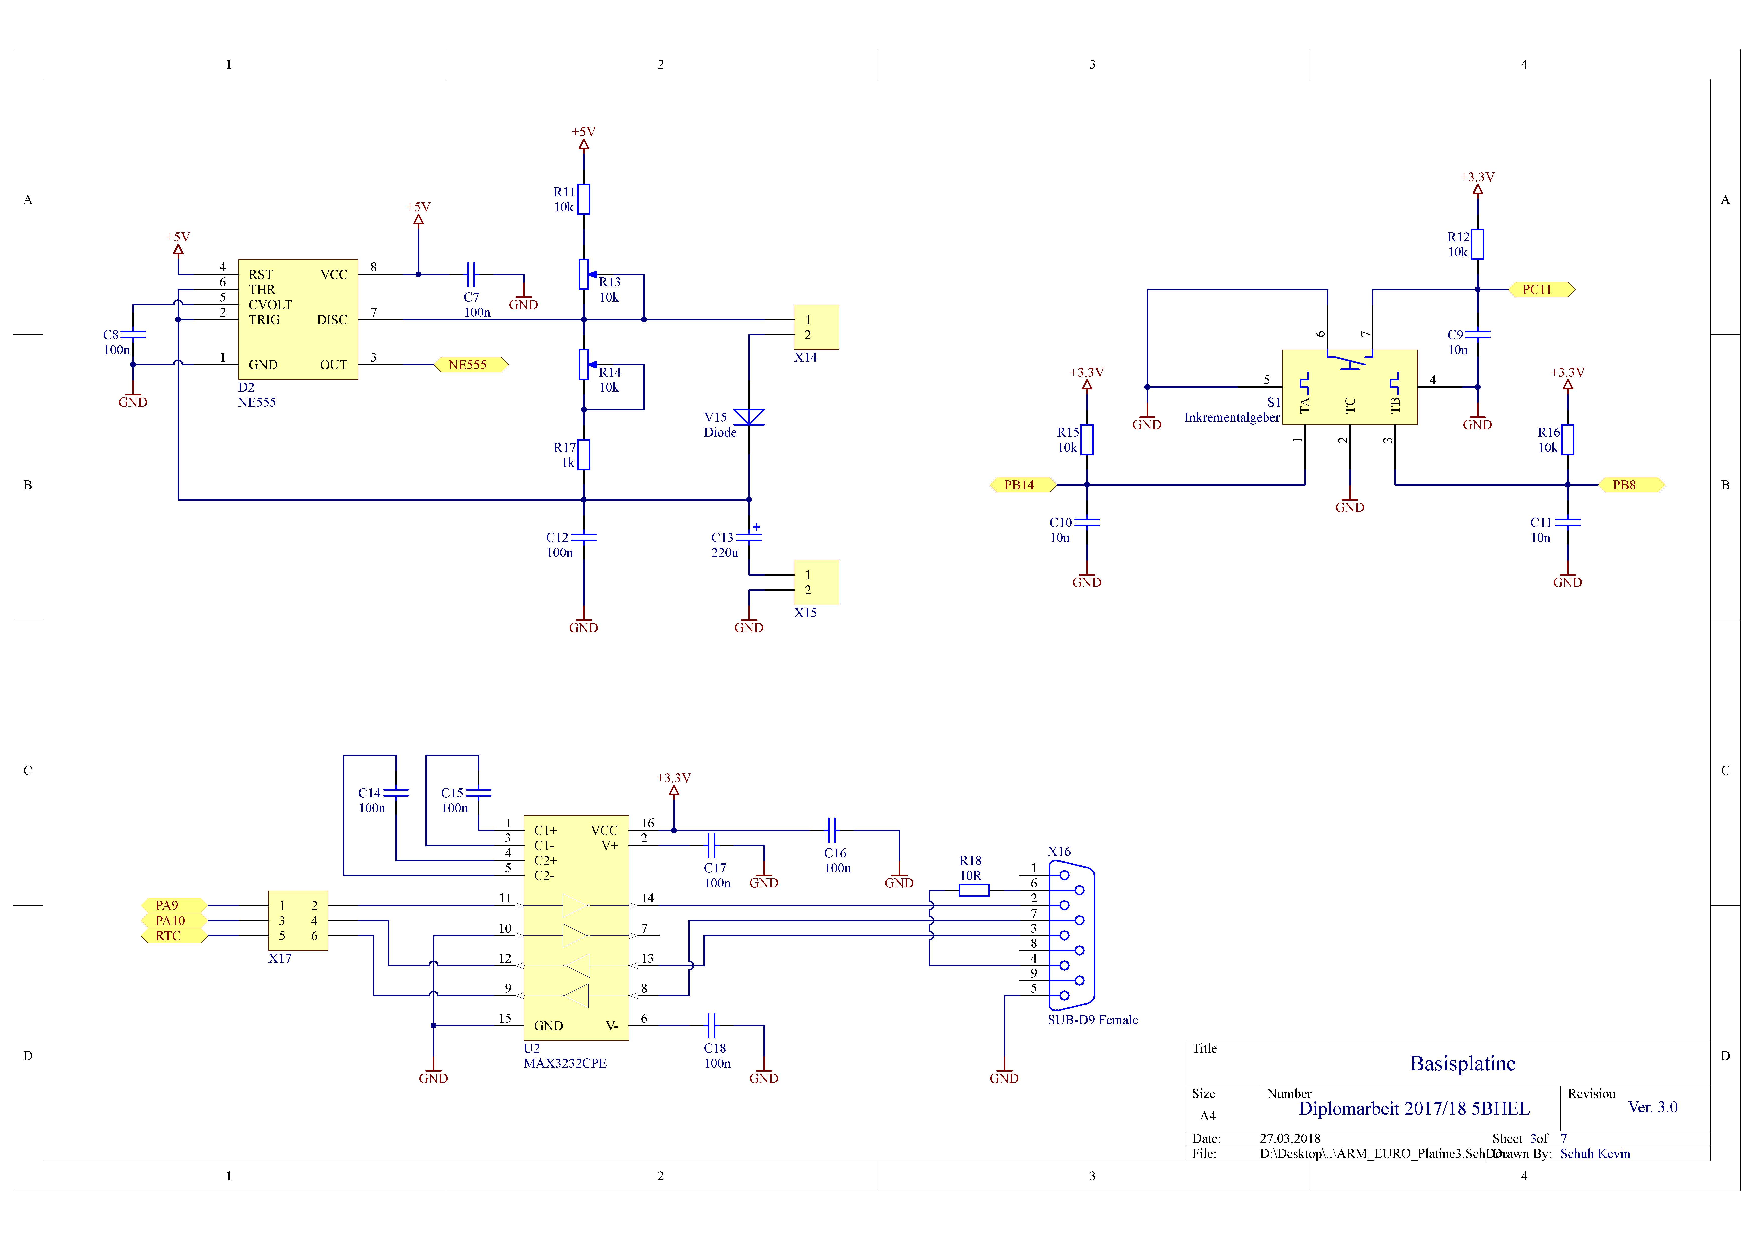
\includegraphics[width=0.8\textwidth]{Schuh/Pictures/Basis-Schaltung3}
    \caption[Gesamtschaltung der Basisplatine]{Gesamtschaltung der \gls{Basisplatine}}
\end{figure}
\begin{figure}[htb]\ContinuedFloat
    \centering
    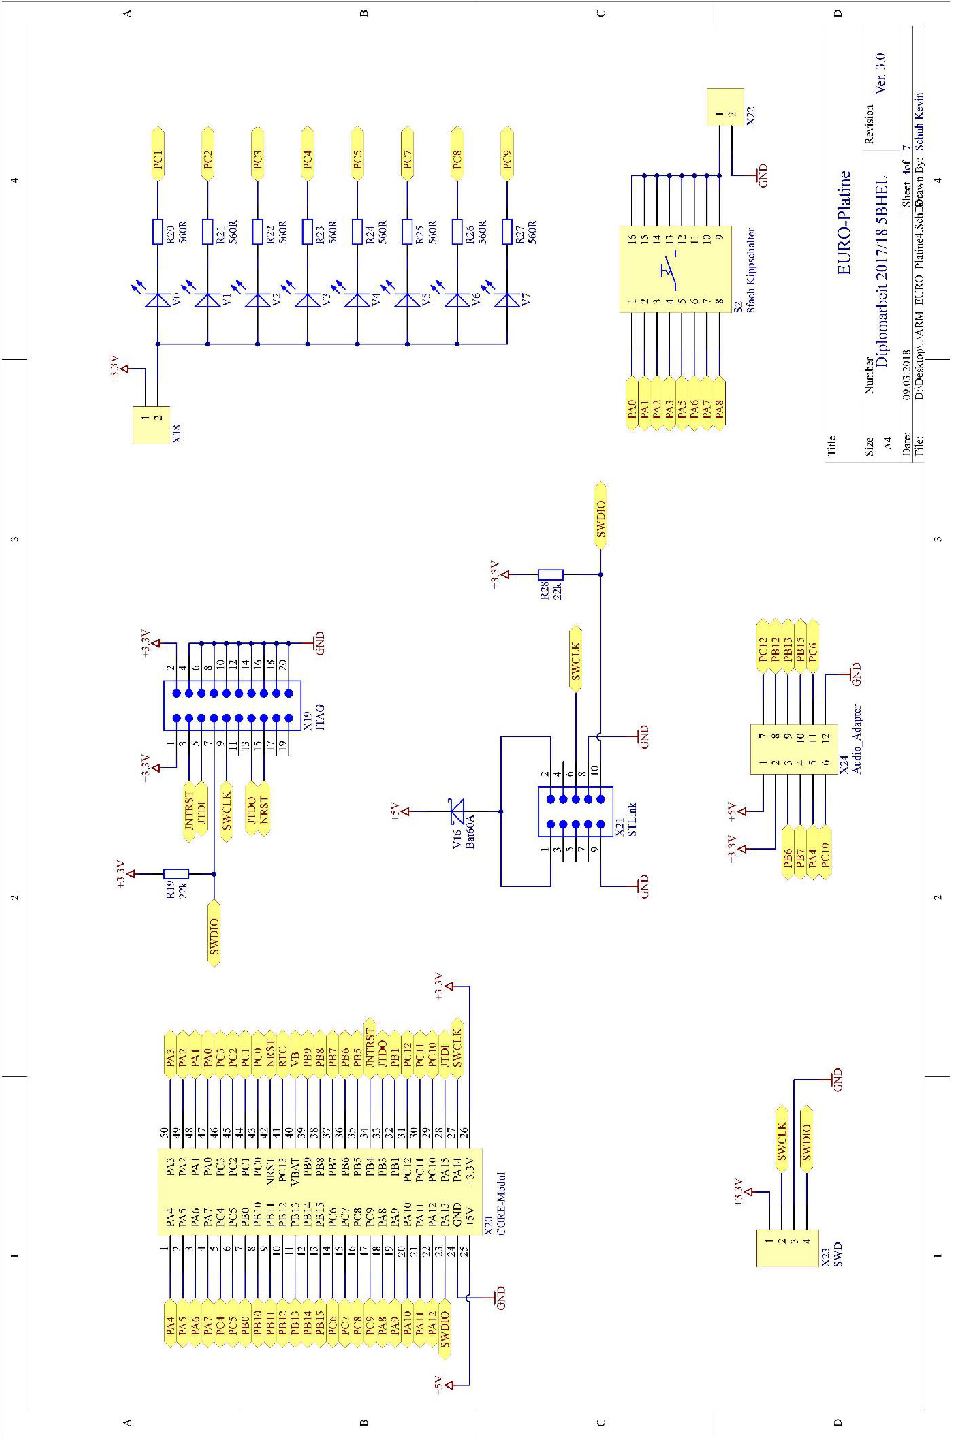
\includegraphics[width=0.8\textwidth]{Schuh/Pictures/Basis-Schaltung4}
    \caption[Gesamtschaltung der Basisplatine]{Gesamtschaltung der \gls{Basisplatine}}
\end{figure}
\begin{figure}[htb]\ContinuedFloat
    \centering
    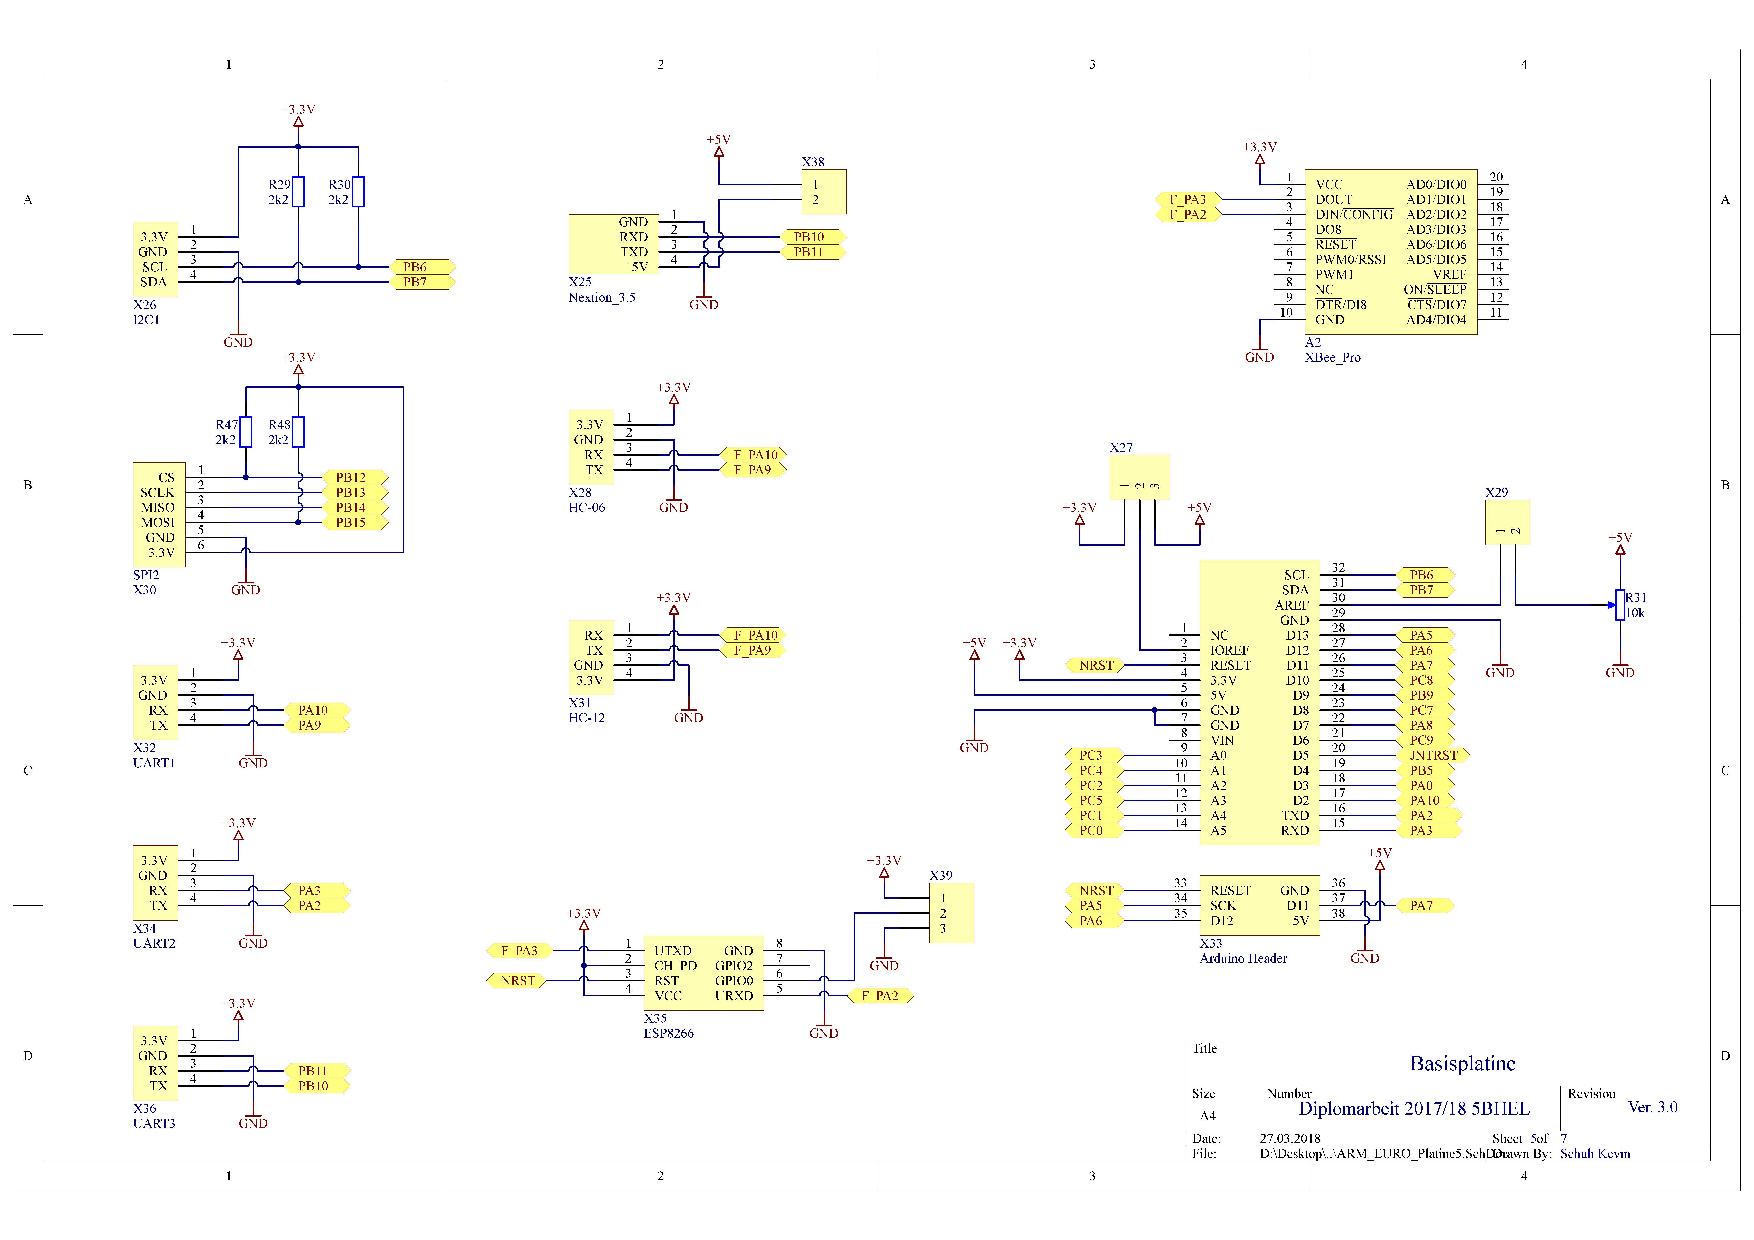
\includegraphics[width=0.8\textwidth]{Schuh/Pictures/Basis-Schaltung5}
    \caption[Gesamtschaltung der Basisplatine]{Gesamtschaltung der \gls{Basisplatine}}
\end{figure}
\begin{figure}[htb]\ContinuedFloat
    \centering
    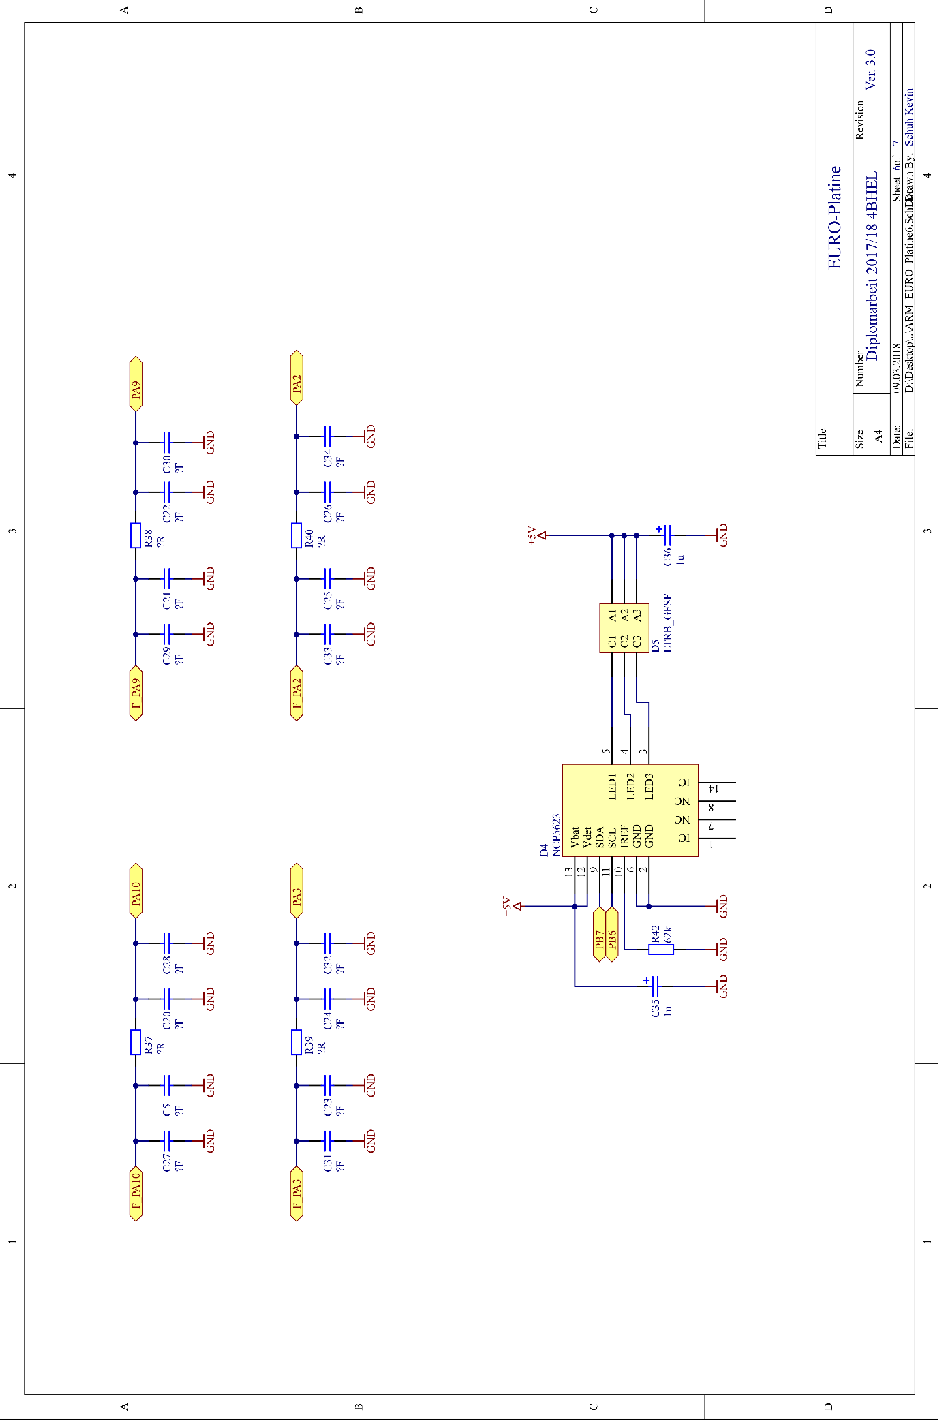
\includegraphics[width=0.8\textwidth]{Schuh/Pictures/Basis-Schaltung6}
    \caption[Gesamtschaltung der Basisplatine]{Gesamtschaltung der \gls{Basisplatine}}
\end{figure}
\begin{figure}[htb]\ContinuedFloat
    \centering
    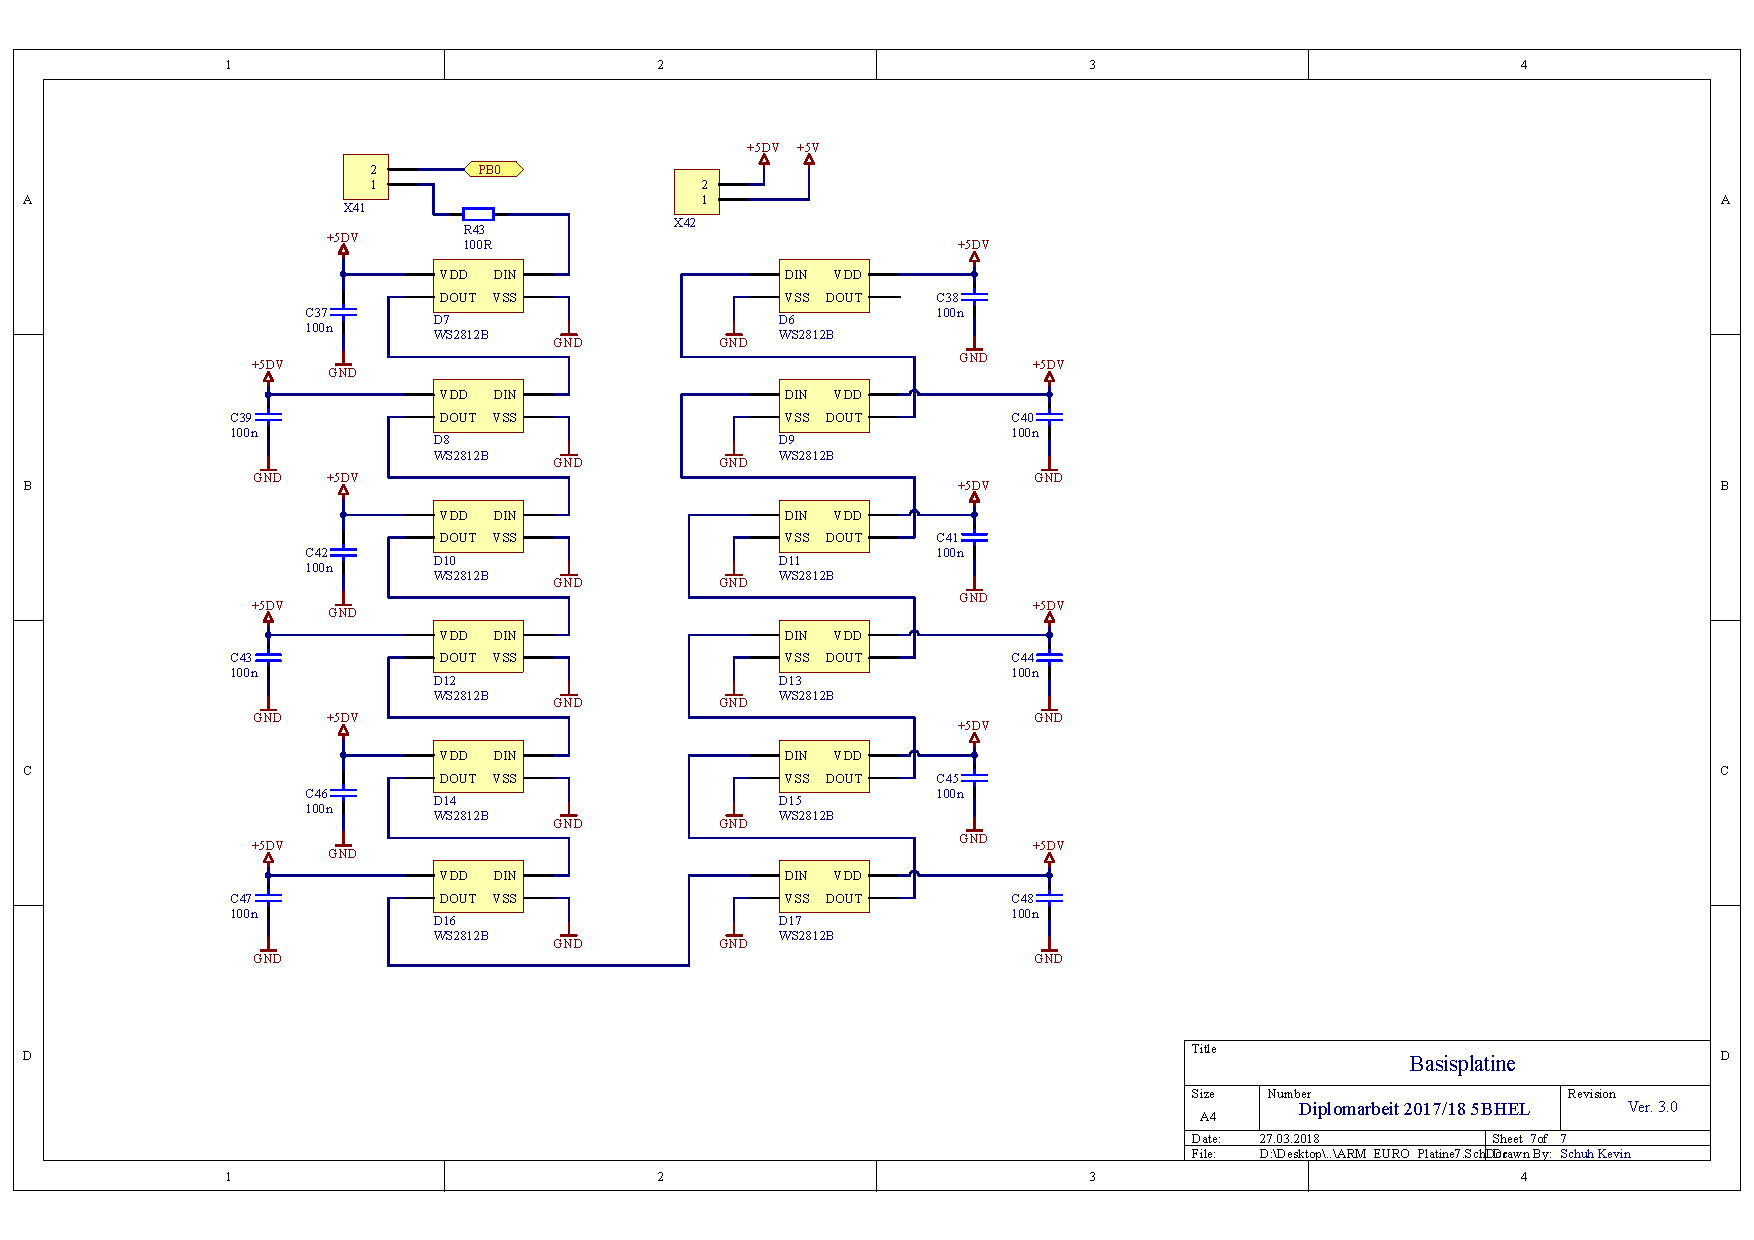
\includegraphics[width=0.8\textwidth]{Schuh/Pictures/Basis-Schaltung7}
    \caption[Gesamtschaltung der Basisplatine]{Gesamtschaltung der \gls{Basisplatine}}
\end{figure}

\subsubsection{ST-Link V2}
\label{sec:basisplatine-stlink}
Zur Programmierung und zum \gls{Debugging} des neuen \gls{ARM}-\gls{Minimalsystem}s sollte ein \textbf{ST-Link V2 Mini} verwendet werden. Dieser Programmer besitzt eine verpolungssichere zweireihige Stiftreihe, welche es ermöglicht Programme mit Hilfe von \gls{SWD} auf den Microcontroller zu übertragen oder diese zu debuggen. Darüber hinaus ist der ST-Link V2 Mini der Lieferant der Hauptversorgungsspannung von \unit{+5}{\volt}.

Um den ST-Link V2 Mini und den Microcontroller im Falle eines Kurzschlusses zwischen der Versorgungsspannung und Masse zu schützen wurde eine Schottky-Diode (\fref{fig:basisplatine-swd}, V16), mit einem maximalen Durchflussstrom von \unit{3}{\ampere}, vorgesehen.

\fig{basisplatine-swd}{ST-Link Schaltung der Basisplatine}{ST-Link Schaltung der \gls{Basisplatine}}{0.6\textwidth}{Schuh/Pictures/Basis-SWD}

\subsubsection{SWD-Adapter}
Der als Buchsenleiste ausgeführte SWD-Adapter (\fref{fig:basisplatine-swd2}, X23), erfüllt vom Prinzip her die gleiche Funktion wie der bereits in \fref{sec:basisplatine-stlink} beschriebene Stecker für den ST-Link V2 Mini. Dieser ermöglicht lediglich Kompatibilität zu anderen SWD-Programmern und Debuggern, welche diesen Stecker nicht besitzen.

\fig{basisplatine-swd2}{SWD-Schaltung der Basisplatine}{\gls{SWD}-Schaltung der \gls{Basisplatine}}{0.5\textwidth}{Schuh/Pictures/Basis-SWD2}

\subsubsection{JTAG}
Zur Programmierung und zum \gls{Debugging} des neuen \gls{ARM}-\gls{Minimalsystem}s wurde aus kompatibilitätsgründen zum alten System zusätzlich vollwertige JTAG-Schnittstelle vorgesehen, um weiterhin mit Hilfe des ULINK/ME Adapters arbeiten zu können. Auch diese Schnittstelle besitzt eine verpolungssichere zweireihige Buchsenleiste (\fref{fig:}, X19), welche es ermöglicht Programme mit Hilfe des JTAG-Protokolls auf den Microcontroller zu übertragen oder diese zu debuggen.

\fig{basisplatine-jtag}{JTAG-Schaltung der Basisplatine}{\gls{JTAG}-Schaltung der \gls{Basisplatine}}{0.5\textwidth}{Schuh/Pictures/Basis-JTAG}

\subsubsection{Core-Modul-Adapter}
Das Schaltplansymbol des \gls{Core-Modul}s (\fref{fig:basisplatine-core}, X20) zeigt das Pinning, welches hardwaremäßig auf den zwei getrennten Buchsenleisten auf der Leiterkarte ausgeführt wurde.

\fig{basisplatine-core}{Core-Modul-Adapter der Basisplatine}{\gls{Core-Modul}-Adapter der \gls{Basisplatine}}{0.5\textwidth}{Schuh/Pictures/Basis-core}

\subsubsection{Audio-Adapter}
Das bereits in einer anderen Diplomarbeit realisierte Audio-Shield kann auf der zweireihigen Buchsenleiste (\fref{fig:basisplatine-audio}, X24) aufgesteckt und anschließend betrieben werden.

\fig{basisplatine-audio}{Audio-Adapter der Basisplatine}{Audio-Adapter der \gls{Basisplatine}}{0.5\textwidth}{Schuh/Pictures/Basis-audio}

\subsubsection{LED-Array}
Auf der \gls{Basisplatine} wurde ein LED-Array realisiert, welches aus acht LEDs besteht und über die Portleitungen (\fref{fig:basisplatine-leds}: PC1 bis PC5 und PC7 bis PC8) angesteuert werden können. Diese LEDs sind in SMD-Form ausgeführt und haben die einheitliche Farbe Grün. Mit Hilfe der Stiftleiste (\fref{fig:basisplatine-leds}, X18) und deinem Jumper können die LEDs aktiviert oder deaktiviert werden. Wenn der Jumper entfernt ist sind die LEDs deaktiviert und die belegten Port-Pins des \gls{Core-Modul}s sind wieder frei verfügbar.

\fig{basisplatine-leds}{LED-Array der Basisplatine}{LED-Array der \gls{Basisplatine}}{0.5\textwidth}{Schuh/Pictures/Basis-leds}

\subsubsection{DIP-Switches}
\label{sec:basis-dip}
Auf der \gls{Basisplatine} wurde ein achtpoliger DIP-Switch realisiert, welcher intern aus acht getrennten Schalten besteht und über die Portleitungen (\fref{fig:basisplatine-dip}: PA0 bis PA3 und PA5 bis PA8) ausgelesen werden kann. Da im Hardwarelayout keine Pullup-Widerstände vorgesehen wurden, muss bei der Programmierung darauf geachtet werden, dass die internen Pullup-Widerstände des Prozessors aktiviert sind. Da jedoch Port Pins PA2 und PA3 mit der UART2-Schnittstelle verbunden sind, erzeugen diese ein Echo, wenn die Schalter S3 und S4 gleichzeitig geschlossen sind. Weiters können durch Jumpern der Stiftleiste (\fref{fig:basisplatine-dip}, X22) alle Schalter im Kippschalter aktiviert oder deaktiviert werden.


\fig{basisplatine-dip}{DIP-Switches der Basisplatine}{DIP-Switches der \gls{Basisplatine}}{0.5\textwidth}{Schuh/Pictures/Basis-dip}

\subsubsection{USB-Varianten und Versorgung über USB}
Die \gls{Basisplatine} unterstützt hardwaremäßig zwei verschiedene USB-Bauformen und drei verschiedene USB-Funktionen. Diese USB-Funktionen sind USB-Device, USB-Host, USB-OTG (on the go) und werden sowohl von der USB-A Buchse (\fref{fig:basisplatine-usb}, X3), als auch von der USB-B Buchse (\fref{fig:basisplatine-usb}, X1) unterstützt. Da beide Buchsenformen keine ID-Leitung besitzen muss für USB-OTG die dafür benötigte Portleitung PA10 mit einem Pullup-Widerstand versehen werden, um den USB-OTG Modus vorzutäuschen. Weiters müssen für den USB-OTG Modus der Pin1 mit dem Pin2 und der Pin3 mit dem Pin4 auf der zweireihigen Stiftleiste (\fref{fig:basisplatine-usb}, X37) gejumpert werden. Über die Portleitung PA10 kann ausgewählt werden ob der Prozessor als USB-Host oder USB-Device arbeitet. Mit der Portleitung PA9 hingegen kann festgestellt werden ob die Versorgung über die USB Buchse funktioniert. Falls man im Host-Modus Geräte ohne Adapter anschließen möchte, wurde eine zweite USB Buchse parallel geschalten.  Sollte man die USB-B Buchse auswählen wollen muss man den Pin1 mit dem Pin3 und dem Pin2 mit dem Pin4 auf der zweireihigen Stiftleiste (\fref{fig:basisplatine-usb}, X2) jumpern. Um die USB-A Buchse auswählen muss man den Pin4 mit dem Pin6 und dem Pin3 mit dem Pin5 auf der zweireihigen Stiftleiste (\fref{fig:basisplatine-usb}, X2) jumpern.

\fig{basisplatine-usb}{USB Buchsen der Basisplatine}{USB Buchsen der \gls{Basisplatine}}{\textwidth}{Schuh/Pictures/Basis-usb}

\subsubsection{Masseschleife}
Um das Messen mit einem Oszilloskop oder anderen Messgeräten zu vereinfachen wurde eine Masseschleife (\fref{fig:basis-masse}, X5) auf der \gls{Basisplatine} realisiert.

\fig{basis-masse}{Masseschleife der Basisplatine}{Masseschleife der \gls{Basisplatine}}{0.25\textwidth}{Schuh/Pictures/Basis-masse}

\subsubsection{Powerswitch STMPS2141}\todo{Quelle?}
Um USB-Geräte zu betreiben, welche selbst keine eigene Spannungsversorgung besitzen (z.B. USB-Sticks) wurde ein Powerswitch (\fref{fig:basisplatine-power}, D3) verbaut. Dieser ermöglicht es die interne \unit{5}{\volt}-Versorgung auf die USB-Buchsen zu legen, damit diese Geräte mit Spannung versorgt werden können. Sollte das Gerät zu viel Strom verbrauchen beginnt die LED (\fref{fig:basisplatine-power}, V9) zu leuchten. Durch Jumpern der Stiftleiste (\fref{fig:basisplatine-power}, X4) an den Port-Pin PC9 kann die Versorgung von externen Geräten gesteuert werden.

\fig{basisplatine-power}{USB Powerswitch der Basisplatine}{USB Powerswitch der \gls{Basisplatine}}{\textwidth}{Schuh/Pictures/Basis-power}

\subsubsection{Powerheader}
Um die auf der \gls{Basisplatine} verwendeten Spannungen direkt für Versuchsaufbauten am Steckbrett oder für externe Sensoren verwenden zu können wurden zwei Buchsenleisten (\fref{fig:basisplatine-pwrhdr}, X6 und X7) ausgeführt, welche diese Spannungen bereitstellen. Dabei ist zu beachten, dass am \unit{12}{\volt}-Ausgang nur \unit{+12}{\volt} anliegen, wenn die Basisplatine über ein externes Netzteil mit einer Ausgangsspannung von \unit{+12}{\volt} betrieben wird. Sollte eine geringere Spannung über das Netzgerät eingespeist werden liegt diese am Ausgang an, wenn hingegen kein Netzteil verwendet wird ist dieser Ausgang spannungsfrei.

\fig{basisplatine-pwrhdr}{Powerheader der Basisplatine}{Powerheader der \gls{Basisplatine}}{0.5\textwidth}{Schuh/Pictures/Basis-pwrhdr}

\subsubsection{\unit{3,3}{\volt}-Versorgung}
Zur Überprüfung ob die \gls{Basisplatine} mit der Betriebsspannung von \unit{+3,3}{\volt} über das \gls{Core-Modul} versorgt wird, wurde die LED (\fref{fig:basisplatine-3v3}, V14) zur optischen Kontrolle eingebaut. Wenn die Basisplatine mit Spannung versorgt wird, beginnt diese zu leuchten.

\fig{basisplatine-3v3}{3,3 V-Versorgung der Basisplatine}{\unit{3,3}{\volt}-Versorgung der \gls{Basisplatine}}{0.25\textwidth}{Schuh/Pictures/Basis-3v3}

\subsubsection{Spannungsversorgung über DC-Buchse}
Die \gls{Basisplatine} unterstützt hardwaremäßig zwei verschiedene USB-Bauformen und drei verschiedene USB-Funktionen. Diese USB-Funktionen sind USB-Device, USB-Host, USB-OTG (on the go) und werden sowohl von der USB-A Buchse (\fref{fig:basisplatine-usb}, X3), als auch von der USB-B Buchse (\fref{fig:basisplatine-usb}, X1) unterstützt. Da beide Buchsenformen keine ID-Leitung besitzen muss für USB-OTG die dafür benötigte Portleitung PA10 mit einem Pullup-Widerstand versehen werden, um den USB-OTG Modus vorzutäuschen. Weiters müssen für den USB-OTG Modus der Pin1 mit dem Pin2 und der Pin3 mit dem Pin4 auf der zweireihigen Stiftleiste (\fref{fig:basisplatine-usb}, X37) gejumpert werden. Über die Portleitung PA10 kann ausgewählt werden ob der Prozessor als USB-Host oder USB-Device arbeitet. Mit der Portleitung PA9 hingegen kann festgestellt werden ob die Versorgung über die USB Buchse funktioniert. Falls man im Host-Modus Geräte ohne Adapter anschließen möchte, wurde eine zweite USB Buchse parallel geschalten.  Sollte man die USB-B Buchse auswählen wollen muss man den Pin1 mit dem Pin3 und dem Pin2 mit dem Pin4 auf der zweireihigen Stiftleiste (\fref{fig:basisplatine-usb}, X2) jumpern. Um die USB-A Buchse auswählen muss man den Pin4 mit dem Pin6 und dem Pin3 mit dem Pin5 auf der zweireihigen Stiftleiste (\fref{fig:basisplatine-usb}, X2) jumpern.

Als weiter Spannungsversorgungsmöglichkeit bietet die \gls{Basisplatine} die Möglichkeit ein \unit{9}{\volt} bis \unit{12}{\volt} DC-Netzteil am die DC-Buchse (\fref{fig:basisplatine-dc}, J1) anzuschließen um die Basisplatine mit Spannung zu versorgen. Der Brückengleichrichter (\fref{fig:basisplatine-dc}, U1) dient dabei lediglich als Verpolungsschutz und nicht als Gleichrichter für Wechselspannung. Das Anlegen von Wechselspannung an die DC-Buchse (\fref{fig:basisplatine-dc}, J1) sollte aus Sicherheitsgründen unterlassen werden. Um aus der hohen Spannung, welche von der DC-Buchse kommt, die Betriebsspannung von \unit{+5}{\volt} zu generieren wurde ein Step-Down Modul (\fref{fig:basisplatine-dc}, U3) der Firma Würth verbaut. Zur Überprüfung ob das Step-Down Modul die Betriebsspannung von \unit{+5}{\volt} generiert, wurde die LED (\fref{fig:basisplatine-dc}, V13) zur optischen Kontrolle eingebaut. Wenn das Step-Down Modul die gewünschte Spannung generiert, beginnt diese zu leuchten. Die Stiftleiste (\fref{fig:basisplatine-dc}, X43) kann im Bedarfsfall gejumpert werden, wenn ein Unterspannungsschutz der Versorgungsspannung gewünscht ist. Um die vom Step-Down Modul generierte Spannung verwenden zu können muss lediglich die Stiftleiste (\fref{fig:basisplatine-dc}, X8) mit einem Jumper versehen werden.

\fig{basisplatine-dc}{DC-Versorgung der Basisplatine}{DC-Versorgung der \gls{Basisplatine}}{\textwidth}{Schuh/Pictures/Basis-dc}

\subsubsection{RGB-LED Ring}
Auf der \gls{Basisplatine} wurde ein aus zwölf RGB-LEDs bestehender Ring aufgebaut, welcher in den verschiedensten Farben leuchten kann. Jede RGB-LED besitzt einen eigenen eingebauten Controller. Die Ansteuerung der LEDs wird über den Port-Pin PB0 realisiert. Um diesen verwenden zu können muss zuvor die Stiftleiste (\fref{fig:basisplatine-ledring}, X41) mit einem Jumper versehen werden. Weiters muss die Spannungsversorgung der LEDs gewährleistet sein. Dazu muss lediglich die Stiftleiste (\fref{fig:basisplatine-ledring}, X42) mit einem Jumper versehen werden.

\fig{basisplatine-ledring}{RGB-LED Ring der Basisplatine}{RGB-LED Ring der \gls{Basisplatine}}{\textwidth}{Schuh/Pictures/Basis-ledring}

\todo{Auslagern nach Theorie? --> Mieke}Zur Programmierung der LEDs muss über den Port PB0 ein Datenwort übetragen werden, welches 24 bit pro LED enthält, siehe \fref{fig:basisplatine-ledring-data}. Dies ergibt insgesamt 288 bit, welche übertragen werden müssen. Wie die Übertragung genau aussieht kann aus \fref{fig:basisplatine-ledring-timing} entnommen werden.

\fig{basisplatine-ledring-data}{RGB-LED Ring Datenstruktur}{RGB-LED Ring Datenstruktur}{\textwidth}{Schuh/Pictures/Basis-ledring-data}
\fig{basisplatine-ledring-timing}{RGB-LED Ring Timing Diagram}{RGB-LED Ring Timing Diagram}{\textwidth}{Schuh/Pictures/Basis-ledring-timing}

\subsubsection{Sensor-Selektion}
Da der verbaute Prozessor zu wenig Portleitungen besitzt um alle Sensoren und Module mit einer eigenen Portleitung zu versorgen, werden einige Portleitungen mehrmals verwendet. Um nun einzelne Module oder Sensoren verwenden zu können, müssen diese einsprechend gejumpert werden. Eine dieser Stiftleisten ist der Header (\fref{fig:basisplatine-ssel}, X9), welches es ermöglicht zwischen einem Potentiometer (\gls{ADC}), Piezo-Summer, einem LFU, einem Infrarotempfänger, einem Temperaturfühler und einem NE555 auszuwählen.

Eine weitere dieser Stiftleisten ist der Header (\fref{fig:basisplatine-ssel2}, X11), welche es ermöglicht zwischen dem Beschleunigungssensor und dem EEPROM auszuwählen.

\fig{basisplatine-ssel}{Sensor-Selektion der Basisplatine}{Sensor-Selektion der \gls{Basisplatine}}{0.5\textwidth}{Schuh/Pictures/Basis-ssel}
\fig{basisplatine-ssel2}{Sensor-Selektion der Basisplatine}{Sensor-Selektion der \gls{Basisplatine}}{0.5\textwidth}{Schuh/Pictures/Basis-ssel2}

\subsubsection{Piezo-Summer}
Auf der \gls{Basisplatine} wurde ein Piezo-Summer (\fref{fig:basisplatine-piezo}, B4) verbaut, welcher über den Port-Pin PB0 angesteuert werden kann. Ja nach anliegender Taktfrequenz am Eingang des Summers wird der erzeugte Ton höher oder tiefer. Um den Piezo-Summer verwenden zu können muss lediglich der Pin11 mit dem Pin12, der zweireihige Stiftleiste (\fref{fig:basisplatine-ssel}, X9), gejumpert werden.

\fig{basisplatine-piezo}{Piezo-Summer der Basisplatine}{Piezo-Summer der \gls{Basisplatine}}{0.5\textwidth}{Schuh/Pictures/Basis-piezo}

\subsubsection{Potentiometer}
Es wurden zwei Potentiometer R9 und R4 hardwaremäßig auf der \gls{Basisplatine} vorgesehen. Diese sind direkt mit einem \gls{ADC}-Eingang des Prozessors verbunden. Der Unterschied zwischen den Potentiometern R9 und R4 besteht darin, dass das Potentiometer R4 über einen Jumper auf der Stiftleiste (\fref{fig:basisplatine-poti2}, X40) aktiviert werden muss und dieses an einem anderen Port-Pin angeschlossen ist. Dieser Aufbau wurde deswegen gewählt da damit, damit an den \gls{ADC}-Eingang auch optional ein anderes Signal angelegt werden kann. 

\fig{basisplatine-poti1}{Potentiometer 1 der Basisplatine}{Potentiometer 1 der \gls{Basisplatine}}{0.5\textwidth}{Schuh/Pictures/Basis-poti1}
\fig{basisplatine-poti2}{Potentiometer 2 der Basisplatine}{Potentiometer 2 der \gls{Basisplatine}}{0.5\textwidth}{Schuh/Pictures/Basis-poti2}

\subsubsection{EEPROM}
Um Daten permanent speichern zu können wurde das EEPROM (\fref{fig:basisplatine-eeprom}, D1) vorgesehen. Standardmäßig wird das EEPROM 24AA256 verwendet, welches es ermöglicht 256 kbit abzuspeichern. Dieses EEPROM besitzt eine Write-Protection WP welche es ermöglicht das EEPROM schreibgeschützt zu schalten. Die Write-Protection kann über die Portleitung PB5 gesteuert werden. Damit das Signal am EEPROM ankommt, muss jedoch der Pin3 mit dem Pin4 der zweireihigen Stiftleiste (\fref{fig:basisplatine-ssel2}, X11) gejumpert werden. Die Kommunikation mit dem EEPROM erfolgt mit dem \IIC{}-Bus.

\fig{basisplatine-eeprom}{EEPROM der Basisplatine}{EEPROM der \gls{Basisplatine}}{0.75\textwidth}{Schuh/Pictures/Basis-eeprom}

\subsubsection{Beschleunigungssensor}
Auf der \gls{Basisplatine} wurde auch ein Beschleunigungssensormodul mit dem Beschleunigungssensor BMA020 vorgesehen. Die Kommunikation mit dem Beschleunigungssensor erfolgt mit Hilfe des \IIC{}-Buses (Adresse \texttt{0x70}). Durch diesen Sensor kann die Neigung, sowie die Kraft welche auf die Platine wirkt in der X, Y und Z-Richtung erfasst werden. Der Beschleunigungssensor besitzt einen Interrupt-Pin, welcher es ermöglicht ein Interrupt auszulösen. Der Interrupt kann über die Portleitung PB5 empfangen werden. Damit das Interrupt-Signal an der Portleitung PB5 ankommt, muss jedoch der Pin1 mit dem Pin2 der zweireihigen Stiftleiste (\fref{fig:basisplatine-ssel2}, X11) gejumpert werden.

\fig{basisplatine-bma}{Beschleunigungssensor der Basisplatine}{Beschleunigungssensor der \gls{Basisplatine}}{0.75\textwidth}{Schuh/Pictures/Basis-bma}

\subsubsection{IR-Receiver}
Um die Platine auch mit einer Fernbedienung oder einem Mobiltelefon steuern zu können würde ein IR-Receiver verbaut. Dieser Sensor wurde hardwaremäßig unter dem NEXTION-Display angebracht. Der IR-Receiver arbeitet mit einer Wellenlänge von 850nm bis 1000nm und einer Trägerfrequenz von 38kHz. Das vom IR-Receiver empfangene Signal wird direkt im Receiver demoduliert und anschließend zu der zweireihigen Stiftleiste (\fref{fig:basisplatine-ssel}, X9) weitergeleitet. Um den IR-Receiver verwenden zu können muss lediglich der Pin7 mit dem Pin8, der Stiftleiste (\fref{fig:basisplatine-ssel}, X9), gejumpert werden.

\fig{basisplatine-ir}{IR-Receiver der Basisplatine}{IR-Receiver der \gls{Basisplatine}}{0.5\textwidth}{Schuh/Pictures/Basis-ir}

\subsubsection{Temperatursensor}
Um die Umgebungstemperatur feststellen zu können wurde auf der Basisplatine der Temperaturfühler DS18B20 verbaut, welcher mit Hilfe des 1-Wire Protokolls angesprochen werden kann. Die maximale Mesfehler dieses Temperatursensors beträgt ±0,5°C laut Datenblattangabe\todo{Quelle?}. Um den Temperaturfühler verwenden zu können muss lediglich der Pin9 mit dem Pin10, der Stiftleiste (\fref{fig:basisplatine-ssel}, X9), gejumpert werden. 

\fig{basisplatine-temp}{Temperatursensor der Basisplatine}{Temperatursensor der \gls{Basisplatine}}{0.5\textwidth}{Schuh/Pictures/Basis-temp}

\subsubsection{Lichtwandler LFU}
Der auf der \gls{Basisplatine} realisierte LFU (Licht-Frequenz-Wandler), wandeltet wie der Name bereits sagt Licht in eine bestimmte Frequenz um. Je höher die Bestrahlungsstärke des Lichts, desto höher wird die über den Output des LFUs ausgegebene Frequenz. Den linearen Zusammenhang zwischen der Bestrahlungsstärke und der ausgegebenen Frequenz kann aus \fref{fig:basisplatine-lfu-freq} entnommen werden.\todo{Quelle?} Um den LFU verwenden zu können muss lediglich der Pin5 mit dem Pin6, der Stiftleiste (\fref{fig:basisplatine-ssel}, X9), gejumpert werden.

\fig{basisplatine-lfu}{LFU der Basisplatine}{LFU der \gls{Basisplatine}}{0.5\textwidth}{Schuh/Pictures/Basis-lfu}
\fig{basisplatine-lfu-freq}{Frequenzgang des LFUs}{Frequenzgang des LFUs}{0.5\textwidth}{Schuh/Pictures/Basis-lfu-freq}

\subsubsection{RGB-LED}
Der auf der \gls{Basisplatine} realisierte LFU (Licht-Frequenz-Wandler), wandeltet wie der Name bereits sagt Licht in eine bestimmte Frequenz um. Je höher die Bestrahlungsstärke des Lichts, desto höher wird die über den Output des LFUs ausgegebene Frequenz. Den linearen Zusammenhang zwischen der Bestrahlungsstärke und der ausgegebenen Frequenz kann aus \fref{fig:basisplatine-lfu-freq} entnommen werden.\todo{Quelle?} Um den LFU verwenden zu können muss lediglich der Pin5 mit dem Pin6, der Stiftleiste (\fref{fig:basisplatine-ssel}, X9), gejumpert werden.

Auf der Hardware der \gls{Basisplatine} wurde eine RGB-LED verbaut, welche mit Hilfe des LED-Divers (\fref{fig:basisplatine-rgbled}, D4), welcher mit dem \IIC{}-Bus angesteuert werden kann. Dieser LED-Driver hat den Vorteil, dass er eine interne Stromüberwachung besitzt. Dadurch benötigen die einzelnen Anoden der RGB-LED keine Vorwiderstände, da sich der Strom automatisch entsprechend der gewünschten Farbe reguliert.

\fig{basisplatine-rgbled}{RGB-LED der Basisplatine}{RGB-LED der \gls{Basisplatine}}{0.5\textwidth}{Schuh/Pictures/Basis-rgbled}
\fig{basisplatine-rgbled-befehl}{Befehlsaufbau der RGB-LED}{Befehlsaufbau der RGB-LED}{\textwidth}{Schuh/Pictures/Basis-rgbled-befehl}
\fig{basisplatine-rgbled-register}{Register der RGB-LED}{Register der RGB-LED}{\textwidth}{Schuh/Pictures/Basis-rgbled-register}
\fig{basisplatine-rgbled-seq}{Sequenzen der RGB-LED}{Sequenzen der RGB-LED}{\textwidth}{Schuh/Pictures/Basis-rgbled-seq}

\subsubsection{Arduino-Shield-Header}
Um Hardware des Arduino-Mikrocontrollersystems nutzten zu können, ohne selbst großen Aufwand in die Entwicklung entsprechender Module investieren zu müssen, wurde ein Arduino-Shield-Header auf der \gls{Basisplatine} vorgesehen. Dieser ermöglicht es durch die Portkompatibilität mit einem Arduino, dessen Shields zu verwenden oder selbst Shields entwickeln zu können. Möchte man nun ein Arduino-Shield verwenden muss dieses lediglich in die vorgesehene Buchsenleiste (\fref{fig:basisplatine-arduino}, X33) gesteckt werden. Da jedes Arduino-Shield die Möglichkeit besitzt eine Referenzspannung für diverse ADCs zu vergeben wurde das Potentiometer R31 vorgesehen, um diesen Spannungspegel variabel zu gestallten. Darüber hinaus gibt es noch die Möglichkeit bei speziellen Shields zu definieren mit welcher Betriebsspannung die darüberliegenden versorgt werden sollen. Dazu wurde die Stiftleiste X27 verbaut, um festzulegen ob die darüberliegenden Shields mit \unit{+5}{\volt} oder \unit{+3,3}{\volt} versorgt werden. Sollte kein Jumper gesetzt werden wird automatisch auf die \unit{+5}{\volt} Spannungsversorgung zurückgegriffen.

\fig{basisplatine-arduino}{Arduino-Shield-Header der Basisplatine}{Arduino-Shield-Header der \gls{Basisplatine}}{\textwidth}{Schuh/Pictures/Basis-arduino}

\subsubsection{WLAN-Modul}
Um Daten ohne großen Aufwand direkt in das Heimnetzwerk einspeisen zu können, wurde auf der auf der \gls{Basisplatine} ein Steckplatz (\fref{fig:basisplatine-wlan}, X35) für ein ESP8266 W-LAN Modul vorgesehen. Dieses Funkmodul benutzt zu Kommunikation mit dem Prozessor des Core-Moduls die UART2 Schnittstelle und sendet die Daten mit einer Sendefrequenz von \unit{2,4}{\giga\hertz} im ISM-Band. Wenn man die Firmware des ESP8266 verändern möchte muss man lediglich die Portleitung GPIO0 des ESP8266, durch jumpern der Pin2 und Pin3 der Stiftleiste (\fref{fig:basisplatine-wlan}, X39), gegen Masse schalten.

\fig{basisplatine-wlan}{WLAN-Modul der Basisplatine}{WLAN-Modul der \gls{Basisplatine}}{0.75\textwidth}{Schuh/Pictures/Basis-wlan}

\subsubsection{XBee-Pro-Modul}
Um Daten ohne großen Aufwand per Funk übertragen können, wurde auf der auf der \gls{Basisplatine} ein Steckplatz (\fref{fig:basisplatine-xbee}, A2) für ein XBee-Pro Modul vorgesehen. Dieses Funkmodul benutzt zu Kommunikation mit dem Prozessor des \gls{Core-Modul}s die UART2 Schnittstelle und sendet die Daten mit einer Sendefrequenz von \unit{2,4}{\giga\hertz} im ISM-Band. Darüber hinaus weist das Funkmodul eine maximale Datenübertragungsrate von 250 kb/s auf und hat eine maximale Reichweite von \unit{1600}{\metre}.

\fig{basisplatine-xbee}{XBee-Pro-Modul der Basisplatine}{XBee-Pro-Modul der \gls{Basisplatine}}{0.5\textwidth}{Schuh/Pictures/Basis-xbee}

\subsubsection{HC-06-Modul}
Um Daten ohne großen Aufwand per Bluetooth übertragen können, wurde auf der auf der \gls{Basisplatine} ein Steckplatz (\fref{fig:basisplatine-hc06}, X28) für ein HC-06 Bluetooth-Modul vorgesehen. Dieses Bluetooth-Modul benutzt zur Kommunikation mit dem Prozessor des \gls{Core-Modul}s die UART1 Schnittstelle und sendet die Daten mit einer Sendefrequenz von \unit{2,4}{\giga\hertz} im ISM-Band. Darüber hinaus weist das Bluetooth-Modul eine maximale Datenübertragungsrate von 1382400 baud auf.

\fig{basisplatine-hc06}{HC-06-Modul der Basisplatine}{HC-06-Modul der \gls{Basisplatine}}{0.5\textwidth}{Schuh/Pictures/Basis-hc06}

\subsubsection{HC-12-Modul}
Um Daten ohne großen Aufwand per Bluetooth übertragen können, wurde auf der auf der \gls{Basisplatine} ein Steckplatz (\fref{fig:basisplatine-hc12}, X31) für ein HC-12 Funkmodul vorgesehen. Dieses Funkmodul benutzt zu Kommunikation mit dem Prozessor des \gls{Core-Modul}s die UART1 Schnittstelle und sendet die Daten mit einer Sendefrequenz von \unit{433,4}{\mega\hertz} bis \unit{473,0}{\mega\hertz} im ISM-Band. Darüber hinaus weist das Funkmodul eine maximale Datenübertragungsrate von 115200 baud auf und hat eine maximale Reichweite von \unit{1800}{\metre}. Das HC-12 Funkmodul kann mittels AT-Befehlen konfiguriert werden. Dabei kann die maximale Ausgangsleistung, die Sendefrequenz und die maximale Datenübertragungsrate verändert werden.

\fig{basisplatine-hc12}{HC-12-Modul der Basisplatine}{HC-12-Modul der \gls{Basisplatine}}{0.5\textwidth}{Schuh/Pictures/Basis-hc12}

Um das Modul in den Programming-Mode zu setzen, müssen folgende Schritte ausgeführt werden:
\begin{itemize}
    \item Um das Modul programmieren zu können muss der Pin5 (\enquote{SET}) gegen Masse gezogen werden, während das Modul mit Spannung versorgt ist (ca. \unit{40}{\milli\second}).
    \item Anschließend muss die Spannungsversorgung unterbrochen werden und der Pin5 (\enquote{SET}) wieder mit Masse verbunden werden. Erst wenn der SET-Pin mit Masse verbunden ist darf das Modul wieder mit Spannung versorgt werden.
\end{itemize}

\tab{basisplatine-hc12-atbefehlsaufbau}{Aufbau von AT-Befehlen}{Aufbau von AT-Befehlen}{|c|p{10cm}|}{
    \hline
    \textbf{Befehl} & \textbf{Funktion}\\
    \hline
    AT & \enquote{AT} ist ein Test-Befehl um festzustellen ob eine Programmierung des Modules möglich ist. Sollte diese möglich sein antwortet das Modul mit \enquote{OK}.\\
    \hline
    AT+B\texttt{xxxx} & Mit diesem Befehl kann die Baudrate des Funkmoduls verändert werden. Anstelle der \enquote{\texttt{x}} gehört die gewünschte Baudrate eingetragen. Sollte der Befehl korrekt an das Funkmodul weitergegeben worden sein antwortet dieses mit \enquote{OK+B\texttt{xxxx}}.\\
    \hline
    AT+C\texttt{xxxx} & Mit diesem Befehl kann der Kommunikationskanal des Funkmoduls verändert werden. Anstelle der \enquote{\texttt{x}} gehört der gewünschte Kommunikationskanal eingetragen. Sollte der Befehl korrekt an das Funkmodul weitergegeben worden sein antwortet dieses mit \enquote{OK+C\texttt{xxxx}}.\\
    \hline
    AT+FU\texttt{x} & Mit diesem Befehl kann der Strombedarf des Funkmoduls verändert werden. Anstelle des \enquote{\texttt{x}} gehört der gewünschte Strombedarf eingetragen. Sollte der Befehl korrekt an das Funkmodul weitergegeben worden sein antwortet dieses mit \enquote{OK+FU\texttt{x}}.\\
    \hline
    AT-P\texttt{x} & Mit diesem Befehl kann die maximale Sendeleistung des Funkmoduls verändert werden. Anstelle des \enquote{\texttt{x}} gehört die gewünschte maximale Sendeleistung eingetragen. Sollte der Befehl korrekt an das Funkmodul weitergegeben worden sein antwortet dieses mit \enquote{OK-P\texttt{x}}.\\
    \hline
    AT-R\texttt{y} & Mit diesem Befehl kann man die aktuellen Einstellungen des Funkmoduls abfragen. Anstelle des \enquote{\texttt{x}} gehört einer der Buchstaben der AT-Befehle (B, C, F, P) eingetragen. Sollte der Befehl korrekt an das Funkmodul weitergegeben worden sein antwortet dieses mit \enquote{OK-R\texttt{y}}.\\
    \hline
    AT+Udps & Mit diesem Befehl können die Anzahl der Datenbits (d), der Paritybits (p) und der Stoppbits (s) verändert werden. Sollte der Befehl korrekt an das Funkmodul weitergegeben worden sein antwortet dieses mit \enquote{OK+Upds}.\\
    \hline
    AT-V & Mit diesem Befehl kann die aktuelle Firmwareversion des Funkmoduls abgefragt werden.\\
    \hline
}
\tabpdf{basisplatine-hc12-at}{HC-12 AT-Befehlsparameter}{Übersicht über die HC-12 AT-Befehlsparameter}{\textwidth}{Schuh/Pictures/Basis-hc12-at}

Um das Funkmodul auf Werkseinstellungen zurückzusetzen muss der AT-Befehl \enquote{AT+DEFAULT} eingegeben werden. Sollte der Befehl korrekt an das Funkmodul weitergegeben worden sein antwortet dieses mit \enquote{OK+DEFAULT}. Um die Firmware des Funkmoduls zu updaten muss der AT-Befehl \enquote{AT+UPDATE} eingegeben werden.

\subsubsection{PI-Filter}
Da die \gls{Basisplatine} auf die Verwendung von Funkmodulen ausgelegt ist, welche im HF-Bereich senden und empfangen, wurden aus Vorsichtsmaßname PI-Filter für die RX- und TX-Leitungen der UARTs, welche mit den Funkmodulen verbunden sind, vorgesehen um HF-Störungen zu unterdrücken. Je nach Bedarfsfall können nun diese PI-Filter bestückt werden. Im laufendem Betrieb hat sich jedoch gezeigt, dass diese nicht unbedingt erforderlich sind.

\fig{basisplatine-pi}{PI-Filter der Basisplatine}{PI-Filter der \gls{Basisplatine}}{\textwidth}{Schuh/Pictures/Basis-pi}

\subsubsection{NEXTION-Display}
Um den Benutzer eine grafische Darstellungsmöglichkeit von Messwerten, Bildern oder ähnlichen zu geben wurde auf der Basisplatine der Header (\fref{fig:basisplatine-nextion}, X25) vorgesehen. Mit Hilfe dieses Headers ist es möglich ein NEXTION-Display auf der Basisplatine zu befestigen und über die UART3-Schnittstelle anzusteuern. Um das NEXTION-Display verwenden zu können muss lediglich die beiden Pins der Stiftleiste (\fref{fig:basisplatine-nextion}, X38) mit einem Jumper verbunden werden. Zur Programmierung des \gls{GUI}, des NEXTION-Displays wird der selbst entwickelte \gls{USB-to-UART}-Adapter benutzt, welcher in \fref{sec:usbtouart}\todo{sec eventuell anpassen} näher erklärt wird.

\fig{basisplatine-nextion}{NEXTION-Display der Basisplatine}{NEXTION-Display der \gls{Basisplatine}}{0.5\textwidth}{Schuh/Pictures/Basis-nextion}

\subsubsection{SPI-Schnittstelle}
Um zusätzliche Hardware mit der \gls{Basisplatine} ansteuern zu können wurde die SPI-Schnittstelle (\fref{fig:basisplatine-spi}, X30) vorgesehen, welche mit der SPI2-Schnitstelle des Prozessors verbunden ist. Da die Chip-Select Leitung (CS) von keiner Hardware auf der Basisplatine benötigt wird, kann diese verwendet werden. Sollten jedoch mehrere Geräte an den SPI-Bus angeschlossen werden, müssen weitere Portleitungen als Chip-Select Leitungen verwendet werden.

\fig{basisplatine-spi}{SPI-Schnittstelle der Basisplatine}{SPI-Schnittstelle der \gls{Basisplatine}}{0.5\textwidth}{Schuh/Pictures/Basis-spi}

\subsubsection{UART-Schnittstelle}
Um zusätzliche Hardware mit der \gls{Basisplatine} ansteuern zu können wurden die Buchsenleiste (\fref{fig:basisplatine-uart}: X32, X34 und X36) realisiert, welche den UART1, UART2, und UART3 des Prozessors verbunden sind. Um eine UART-Schnittstelle verwenden zu können ist es wichtig die RX- und TX-Leitung im Vergleich zum verwendeten Modul zu vertauschen (Null-Modem-Kabel). Alle verwendeten UART-Schnittstellen wurden aus der Sicht des Prozessors bezeichnet.

\begin{warning}
    Anmerkung: Bei der Verwendung der UART2-Schittstelle ist Vorsicht geboten, da wie bereits in \fref{sec:basis-dip} beschrieben, ein Echo auf der Schnittstelle ausgelöst wir, wenn die Kippschaltschalter S3 und S4 gleichzeitig geschlossen sind.
\end{warning}

\fig{basisplatine-uart}{UART-Schnittstelle der Basisplatine}{UART-Schnittstelle der \gls{Basisplatine}}{0.25\textwidth}{Schuh/Pictures/Basis-uart}

\subsubsection{\IIC{}-Schnittstelle}
Um über die \gls{Basisplatine} weitere \IIC{} Geräten anschließen zu können wurde die Buchsenleiste (\fref{fig:basisplatine-iic}, X26) vorgesehen. Die Anschlüsse sind direkt mit der \IIC{}1 Schnittstelle des Mikrocontrollers verbunden. Die \IIC{}-Schnittstelle verfügt über zwei PullUp-Widerstände, da der verwendete Mikrocontroller PullUp-Widerstände nur im Input-Modus zur Verfügung stellt.

\fig{basisplatine-iic}{\IIC{}-Schnittstelle der Basisplatine}{\IIC{}-Schnittstelle der \gls{Basisplatine}}{0.5\textwidth}{Schuh/Pictures/Basis-iic}

\subsubsection{Inkrementalgeber}
Um einfache Regelaufgaben oder Auswahlaufgaben realisieren zu können wurde auf der \gls{Basisplatine} ein Inkrementalgeber vorgesehen. Dieser verfügt über einen Taster, welcher über die Portleitung PC11 abgefragt werden kann. Darüber hinaus kann mit Hilfe der Portleitungen PB8 und PB14 festgestellt werden in welche Richtung und um wie viele Schritte der Inkrementalgeber gedreht wurde. Eine komplette Umdrehung des Inkrementalgebers setzt sich aus 24 Einzelschritten zusammen.

\fig{basisplatine-ink}{Inkrementalgeber der Basisplatine}{Inkrementalgeber der \gls{Basisplatine}}{0.75\textwidth}{Schuh/Pictures/Basis-ink}
\fig{basisplatine-ink-timing}{Inkrementalgeber Timing-Diagramm}{Inkrementalgeber Timing-Diagramm}{\textwidth}{Schuh/Pictures/Basis-ink-timing}

\subsubsection{Serielle Schnittstelle}
Um mit Messgeräten oder PCs zu kommunizieren unterstützt die \gls{Basisplatine} eine Serielle-Schnittstelle. Für diese Schnittstelle wird der UART1 des Prozessors verwendet. Die Pegelumwandlung, von $\pm$\unit{12}{\volt} auf \unit{3,3}{\volt}, welche für die Kommunikation benötigt werden erfolgt mit Hilfe eines MAX232. Die Portleitung PC13 (Tamper-RTC) kann als Handshakeleitung verwendet werden. Zur Verwendung der Seriellen-Schnittstelle, ohne Handshake-Leitung, muss lediglich der Pin1 mit dem Pin2 und der Pin3 mit dem Pin4, der Stiftleiste (\fref{fig:basisplatine-rs232}, X17) miteinander mit Hilfe eines Jumpers verbunden werden. Sollte man die Handshake-Leitung verwenden möchten, muss lediglich der Pin5 mit dem Pin6, der Stiftleiste (\fref{fig:basisplatine-rs232}, X17) miteinander verbunden werden.

\fig{basisplatine-rs232}{Serielle Schnittstelle der Basisplatine}{Serielle Schnittstelle der \gls{Basisplatine}}{\textwidth}{Schuh/Pictures/Basis-rs232}

\subsubsection{NE555}
Der auf der \gls{Basisplatine} verbaute NE555 kann als externer Taktgenerator verwendet werden. Die Periodendauer von diesen, kann mit Hilfe des Verhältnisses der beiden Potentiometer (\fref{fig:basisplatine-ne555}, R13 und R14) verändert werden. Für die Realisierung von großen Zeitkonstanten, kann man durch verbinden der beiden Pins auf der Stiftleiste (\fref{fig:basisplatine-ne555}, X15), mit einem Jumper, einen größeren Kondensator (\fref{fig:basisplatine-ne555}, C13) parallel zum kleineren Kondensator (\fref{fig:basisplatine-ne555}, C12) schalten. Möchte man einen kleineren Widerstand erzielen, kann man das durch einen Jumper auf der Stiftleiste (\fref{fig:basisplatine-ne555}, X14) erzielen. Um den NE555 verwenden zu können muss lediglich der Pin11 mit dem Pin12, der Stiftleiste (\fref{fig:basisplatine-ssel}, X9), mit einem Jumper verbunden werden.

\fig{basisplatine-ne555}{NE555 der Basisplatine}{NE555 der \gls{Basisplatine}}{0.75\textwidth}{Schuh/Pictures/Basis-ne555}

Die Gesamtperiodendauer des NE555 setzt sich aus Summe der Teilperiodendauern t1 und t2 zusammen, kann jedoch auch direkt berechnet werden. Die Formeln zu Berechnung der Periodendauer lauten wie \fref{eq:ne555} zeigt, \fref{fig:basisplatine-ne555-timing} stellt die Beziehung der Werte zueinander grafisch dar.

\fig{basisplatine-ne555-timing}{Timing des NE555}{Timing des NE555}{0.75\textwidth}{Schuh/Pictures/Basis-ne555-timing}

\eq{ne555}{
    \begin{split}
    T & = t_1 + t_2 = 0,7 * [1k\Omega + R_13 + 2 * R] * C \\
    t_1 & = 0,7 * (1k\Omega + R_13 + R) * C \\
    t_1 & = 0,7 * R * C
    \end{split}
}

Der Kondensatorwert C entspricht bei nicht gejumperter Stiftleiste (\fref{fig:basisplatine-ne555}, X15), den Kondensatorwert von C12 (\unit{100}{\nano\farad}). Sollte die Stiftleiste jedoch gejumpert sein, entspricht der Kondensatorwert von C dem Kondensatorwert der Parallelschaltung des Kondensators C12 und C13 (\unit{220,1}{\micro\farad}). Möchte man einen Tastgrad von 0,5 erzielen, muss lediglich die Stiftleiste (\fref{fig:basisplatine-ne555}, X14) gejumpert werden. Wenn diese nicht gejumpert wird ergibt sich der Widerstand R aus der Summe von R14 und R17.

\subsection{Leiterplattenlayout}
\label{sec:basisplatine-leiterplattenlayout}
\subsubsection{Bauteilseite}
\fig{basisplatine-lbauteilseite}{Layout Bauteilseite der Basisplatine}{Layout Bauteilseite der \gls{Basisplatine}}{\textwidth}{Schuh/Pictures/Basis-lbauteilseite}

\subsubsection{Lötseite}
\fig{basisplatine-llötseite}{Layout Lötseite der Basisplatine}{Layout Lötseite der \gls{Basisplatine}}{\textwidth}{Schuh/Pictures/Basis-llotseite}

\subsection{Bestückungspläne}
\label{sec:basisplatine-bestückungspläne}
\subsubsection{Bauteilseite}
\fig{basisplatine-bbauteilseite}{Bestückungsplan Bauteilseite der Basisplatine}{Bestückungsplan Bauteilseite der \gls{Basisplatine}}{\textwidth}{Schuh/Pictures/Basis-bbauteilseite}